\documentclass{article}

\usepackage[final,nonatbib]{nips_2017}

\usepackage[utf8]{inputenc} % allow utf-8 input
\usepackage[T1]{fontenc}    % use 8-bit T1 fonts
\usepackage{hyperref}       % hyperlinks
\usepackage{url}            % simple URL typesetting
\usepackage{booktabs}       % professional-quality tables
\usepackage{amsfonts}       % blackboard math symbols
\usepackage{nicefrac}       % compact symbols for 1/2, etc.
\usepackage{microtype}      % microtypography

\usepackage[backend=biber]{biblatex}
\addbibresource{re-reika.bib}

\usepackage{graphicx}
\graphicspath{ {images/} }

% https://tex.stackexchange.com/questions/376420/include-chinese-characters-into-article-in-xelatex
\usepackage{fontspec}
\newfontfamily\cjkfont{Noto Sans CJK SC}

\usepackage{listings}

\title{Re-Reika: Engineering a DSL compiler}

\author{
Pinglei Guo \\
\texttt{piguo@ucsc.edu}
}

\begin{document}

\maketitle

\begin{abstract}
    % TODO: update abstract
    A compiler for DSL
\end{abstract}

\section{Introduction}
\label{sec:introduction}

\subsection{Motivation and Accomplishment}
\label{subsec:motivation}

We decided to continue the development of Reika \footnote{\url{https://github.com/xephonhq/tsdb-proxy-java/tree/master/ql}},
a DSL for time series database previously built in CMPS203.
\footnote{\href{https://github.com/xephonhq/tsdb-proxy-java/blob/master/ql/Reika\_TSDB\_DSL\_0.0.1.pdf}{Reika\_TSDB\_DSL\_0.0.1.pdf}}.
However, in this quarter, we mainly focused on more detailed design (type system etc.)
and how to make the compiler extensible and maintainable.
Also we no longer limit it to time series data, we want it to be able to handle common data analytic tasks, even simple machine learning.

Due to the duration of the quarter, half of the time was spending on survey and building small prototype.
A survey of q, juila, kotlin, groovy, scala, dotty, weld~\cite{palkar2017weld}'s design and compiler implementation is listed in \verb+doc/dev-notes/at15+.
We implemented simply typed lambda calculus (\verb+simplebool+) and preceding exercises from TAPL in Java.
\footnote{located in tapl folder}
A typecheker, interpreter and transpiler for \verb+SimpleBin+ (only has int and boolean) \footnote{located in playground package of Reika}
to demonstrate how our real implementation is structured and the relation ship between typechecker, interpreter and transpiler.
The real Reika implementation is written from scratch without using old Reika codebase,
and because of a major refactor in the middle \footnote{\url{https://github.com/at15/reika/pull/31}} due to design flaw in AST and compiler phases, the latest version is currently stuck on
\verb+namer+ (symbol and scope) and \verb+typechecker+ phases,
it will be continued and integrate into author's master thesis during winter break and final quarter.

\subsection{Why Reika DSL instead of Python or SQL}
\label{subsec:why-reika}

A common question asked by friends of mine is why don't you just use python,
which is widely used in big data and machine learning as glue language.
The reason is python is not statically typed and it has a lot of legacy,
even though 3.6 adds type hint, most libraries don't have it, not to mention those struggle between python2 and python3.
When you run a python program,
it can execute 999 lines but throw error at last line because you concat a int to string when you try to save the result.

Languages like SQL is typed, but it is checked against schema until it is sent to server,
we want error when I typed invalid column name in editor.
Also there is always a layer of conversion between SQL query result and the code you used to implement bossiness logic
like generating report and graph, extra check is needed everywhere, they should be unified.

We want a language for data analytic that fails fast, has good editor integration.
It should be interactive for exploration and have good performance when run in production.
Which leads to our statically typed, mostly declarative DSL - Reika.
The rest of the paper is organized as following,
Section~\ref{sec:design} describes current syntax and semantic,
the choice we made in our type system and the overview of the compiler structure.
Section~\ref{sec:implementation} shows the progress so far and specific problems we have solved.
Section~\ref{sec:related-work} list related work and our difference with them.
Section~\ref{sec:future-work} contains the priority of unfinished work and potential new features.
Section~\ref{sec:conclusion} concludes the paper.

\section{Design}
\label{sec:design}

\subsection{Syntax}
\label{subsec:syntax}

The new syntax of Reika is mainly modeled after Q\footnote{http://code.kx.com/q/},
and syntax from Java-like language to make it easier to learn and maintain.
In Q, list and record are basic data structure, the underlying database can be represented as (flip of) a record of list,
how the data is actual stored on disk and memory is hidden to the user\footnote{Q is not open source}.
We do not use indent to structure code, because it makes parser easier implement, also code format is easier to do as well.
\footnote{We are using parser generator ANLTR, which is already pretty easy, but there is no harm to reduce complexity}
Semicolon is used to split expressions and curly brackets are used to group expression together for function and control blocks.

% FIXME: there is no ident for function
\texttt{/* \\
@author: at15 \\
@time: 2017-12-15 \\
*/ \\
val x:Int = 1; \\
val y:List[Int] = x + [1, 2, 3]; // [2, 3, 4]:List[Int] \\
plot([1,2,3], y) // a graph shows in browser \\
func a(x:Int, y:Int): Int \{ x + y; \} \\
val z = a(x, 2); // 3:Int \\
\\
val months = [1:5]; // [1, 2, 3, 4, 5] \\
val incomes = 5 rand\_from [10, 25]; // [10, 25, 25, 10, 10] \\
val account\_book = make\_table(\{ months: months, incomes: incomes \}); \\
print(account\_book); \\
| months | incomes | \\
|   1    |   10    | \\
|   2    |   25    | \\
val m = select max(incomes) from account\_book; // 25:Int\\
val ms = select months, incomes from account\_book where incomes > 10; // {months: [2. 3], incomes: [25, 25]} \\
val ms2 = ms.incomes + m // {months: [2. 3], incomes: [50, 50]} \\
\\
val stock: \{tm: List[Date], price: List[Float], symbol: List[String]\} = read\_csv("2016-Jan-01-stocks.csv") \\
% TODO: https://stackoverflow.com/questions/7745609/sql-select-only-rows-with-max-value-on-a-column
val company = select symbol from stock where price is max(price); // AAPL:String
}

Above shows the syntax of new Reika (not fully implemented).
As you may noticed, type can be omitted in several places except function parameters, and variables are not mutable.
Add operator can broadcast (is overloaded) \texttt{1 + [1, 1]} is interpreted as \texttt{[1, 1] + [1, 1]}.
SQLish query can be executed on record of list after it is converted to table,
and data can be read from file or other data source, validation and conversion is performed by the runtime.

\subsection{Type System}
\label{subsec:type-system}

\subsubsection{No Type Inference}
\label{subsubsec:no-type-inference}

As a statically typed language, we chose to explict specify type instead of rely on syntax and inference.
The main reason is we want to support overloading (ad-hoc polymorphism), so we can write 1 + [1, 2, 3] instead of 1 +l [1, 2, 3].
This is more like a syntax sugar because it is resolved at compile time for performance.
However, it's hard to do type inference when overloading is involved (same syntax structure can result in multiple constraints),
the type system in Reika is quite limited, so we chose overload over type inference.

However, even without type inference, type specification can be omitted in certain places,
variable don't need to explict specify type (i.e. \verb+val x = 1+ instead of \verb+val x:Int = 1+)
because it can be computed from right hand side (like C++'s new \verb+auto+ keyword).
This is \textbf{not} type inference in ML languages like OCaml, Haskell.
The difference between compute type and inference type has confused me a lot (before taking the course).
From implementation side, compute type just need one pass, while inference need two pass, one for generating constraint, one for solve it (unification).
Considering the following lambda calculus (sort of) example:

\begin{center}
    ($\lambda$ x. y = x + 1) and ($\lambda$ x:Int. y = x + 1)
\end{center}

The first one need type inference for y while the second one just compute the type
because the first one has variable \verb+x+ with unbounded type.
The only way to introduce variable (w/ or w/o type) is using function (declaring variable in global space can be think
as the entire program is a function), so as long as the function parameter has type, you don't need type inference, you just
simply compute the type because there won't be variable with unbounded type on 'rhs'.
\footnote{TODO: it should be proved, could be wrong, but a quarter is too short for making things sound}

But we still suggest user putting type even when it not necessary needed, because it serves as documentation,
if you write \verb+val x =+ and went for a coffee, you might not remember what you were trying to do 5 mins ago,
but if you write \verb+val x:Int =+, it is a cache that limit the search domain in your head.
This also applies to large projects as well, it is much better than writing a comment \verb+/* x is int*/ val x = 1.0+.
Documentation can't keep up with the rapid iteration, but compiler can, it will throw error you if you write \verb+val x:Int = 1.0+.

\subsubsection{Type check with external data source}
\label{subsubsec:type-check-with-extrenal-data-source}

Since one of our motivation is to fail early, all operation related with external data source such as file, database
are paid extra attention.
Before running the actual code, the runtime would try to valid all the data source are available and has the right type
\footnote{TODO: there should be formal name and existing implementation in literature, but I didn't find any so far},
i.e. a csv file should exists, and can contains more column but not less (subtype),
and the type should match what the user specified.
Normally, user have to implement those guardian code in languages like python, and a lot of time I find it verbose and repetitive.
So we decide to put it into the language.
However, we don't allow pass type to function, so it should be a hack in compiler implementation,
where data source related built in function need to look at the left hand side for expected type.
The reverse of this (kind of) is known as information based programming in F\# \footnote{http://thorium.github.io/FSharpAzure/2-DataUsage/DataUsageEng.html}.
It might be possible to do similar in Reika, use \texttt{type Stock = load\_type\_from\_csv("2016-Jan-01-stocks.csv")},
those two does not has conflict, one is eager runtime check, another is type system aided by data source at compile (develop) time
(the data source must be reachable when compile).

\subsection{Compiler Architecture}
\label{subsec:compiler-architecture}

Previous design and implementation of Reika targets query language like SQL, making its compiler simple.
Symbol and type checking are put into single traverse when constructing AST from parse tree.
The interpreter then execute AST to get the result, there is no user defined function and variable is mutable.
And since user can't define function, everything is implemented in host language and provided as builtin,
the is not concept like package or module.
However, since we want to make Reika more general, the old design is too restrictive.

\begin{center}
  \verb+REPL/file+ > \verb+ANTLR(lexer&Parser)+ > \verb+Symbol&Type(AST)+ > \verb+Interpreter+
\end{center}

The new design of Reika allow user to define function, and part of standard library is written in Reika,
reduce the burden of the host language when porting.
And this forces us to split symbol and type checking from constructing AST and do it in multiple phases.

\begin{figure}[h]
    \centering
    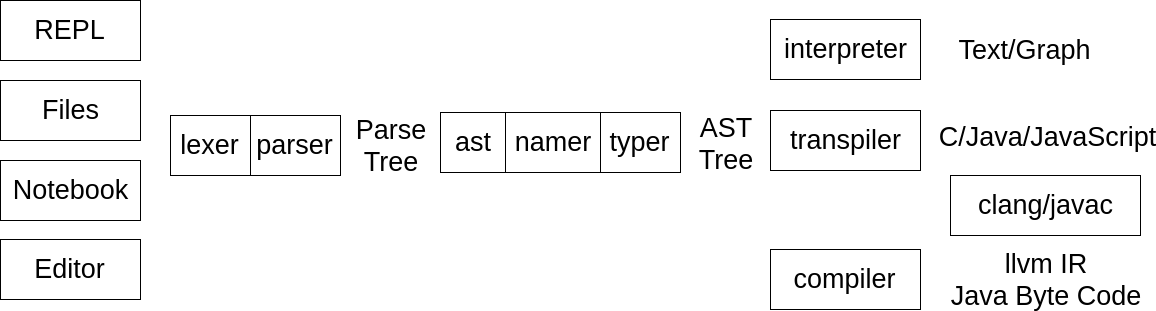
\includegraphics[width=\columnwidth]{reika-compiler}
    \caption{New Reika Compiler design}
    \label{fig:reika-compiler}
\end{figure}

As shown in figure~\ref{fig:reika-compiler}, its input can also be notebook or editor,
so it should be able to start a compiler server and do compile incrementally,
also using a compiler server increase compile speed even without incremental compile when we wrote compiler in language with JIT.
Extra phase (\verb+ast+) after parser is needed because we only get a Parse Tree after using ANLTR, and we need a cleaner AST.
The typed AST can go three directions (in parallel).
For interpreter, it gives back text and graph directly.
For transpiler, based on code template, the AST is converted to C/Java/JavaScript,
target language need to have standard library implemented, external compiler is called to compile the generated code.
For compiler, we can generate LLVM IR or Java Byte Code directly, skipping the call to external compiler,
though since it's hard to do the optimization right, it might be better to sacrifice compile time for correctness and runtime performance.


% TODO: multi dialect
% TODO: Syntax, Type System
% TODO: unify compiler, interpreter, transpiler
% TODO: 伪编译语言算不算编译语言? - 梨梨喵的回答 - 知乎
% https://www.zhihu.com/question/263559593/answer/270924481
% 二村射影 https://en.wikipedia.org/wiki/Partial_evaluation
% TODO: phases, parallel phases (immutable trees)

\section{Implementation}
\label{sec:implementation}

% TODO: several stages, TAPL, SimpleBin, Typed Reika
% lexer, handling negative number

\section{Related Work}
\label{sec:related-work}

% TODO: weld
% TODO: RezzoomSQL
% TODO: Dotty, Groovy

\section{Future Work}
\label{sec:future-work}

\section{Conclusion}
\label{sec:conclusion}

\printbibliography

\end{document}
